\documentclass[journal=jacsat,manuscript=article]{achemso}
\usepackage[version=3]{mhchem}
\usepackage{amsmath}
\usepackage{ctex}
\usepackage{longtable}
\usepackage{booktabs}
\newcommand*\mycommand[1]{\texttt{\emph{#1}}}
\providecommand{\tightlist}{%
  \setlength{\itemsep}{0pt}\setlength{\parskip}{0pt}}
\author{蓝海}
\altaffiliation{我们认真科学分析金融的规律}
\email{lh_loki@163.com}
\phone{13127900572}
\author{彭莉}


\keywords{资深,管理型}

\title[洪流]{洪流简评\footnote{详尽的数据分析与记录请联系作者索取《基金管理人分析技术文档》}}
\makeatletter
\ifxetex
  \usepackage[setpagesize=false, % page size defined by xetex
              unicode=false, % unicode breaks when used with xetex
              xetex]{hyperref}
\else
  \usepackage[unicode=true]{hyperref}
\fi
\hypersetup{breaklinks=true,
            bookmarks=true,
            pdfauthor={},
            pdftitle={},
            colorlinks=true,
            urlcolor=blue,
            linkcolor=magenta,
            pdfborder={0 0 0}}
\urlstyle{same}  % don't use monospace font for urls
% pandoc header

\begin{document}
\begin{abstract}
洪流是资深的投资人。他具备数学本科的背景,工作经历上提供了完整的管理能力、资产配置能力与资管能力的训练,同时形成了一个强大的朋友圈,因此成就了他深度行业分析与配置能力,较强的择股能力。同时他也具备强大的气质和管理经验,是一位成熟的基金经理的经理。
基于公开信息分析,我们认为洪流能够驾驭多种不同的投资风格,适应复杂的市场环境的,具备独到的研究能力和管理能力的首席投资官。
\end{abstract}
\begin{figure}[htbp]
\centering
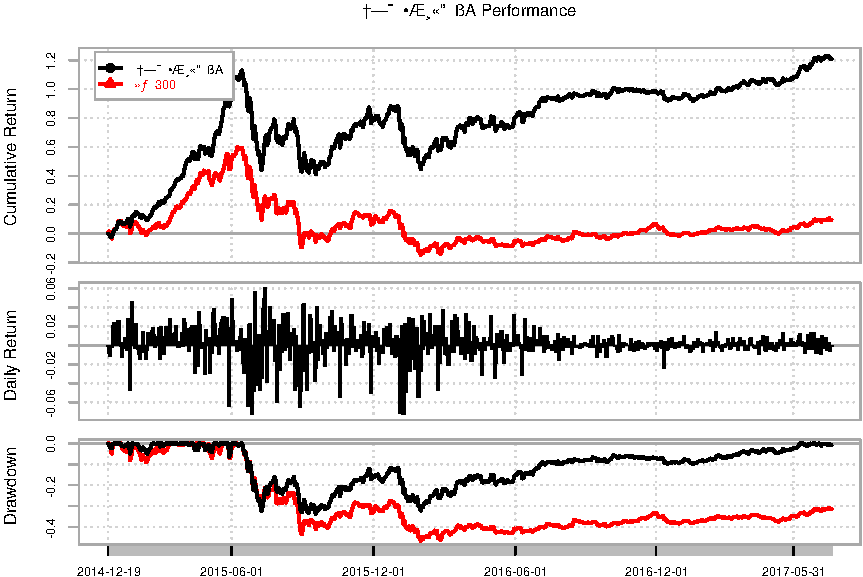
\includegraphics{hl-review_files/figure-latex/unnamed-chunk-2-1.pdf}
\caption{基金累计回报率与回撤}
\end{figure}

\begin{longtable}[]{@{}llclclclc@{}}
\toprule
名称 & 近半年 & 夏普率 & 近一年 & 夏普率 & 两年 & 夏普率 & 三年 &
夏普率\tabularnewline
\midrule
\endhead
圆信永丰双红利A & 12.3\% & 2.6 & 18\% & 1.5 & 8.3\% & 0.05 & 121\% &
1.18\tabularnewline
沪深300 & 8.9\% & 1.6 & 16\% & 1.2 & -28.6\% & -0.62 & 14\% &
0.05\tabularnewline
\bottomrule
\end{longtable}

\begin{figure}[htbp]
\centering
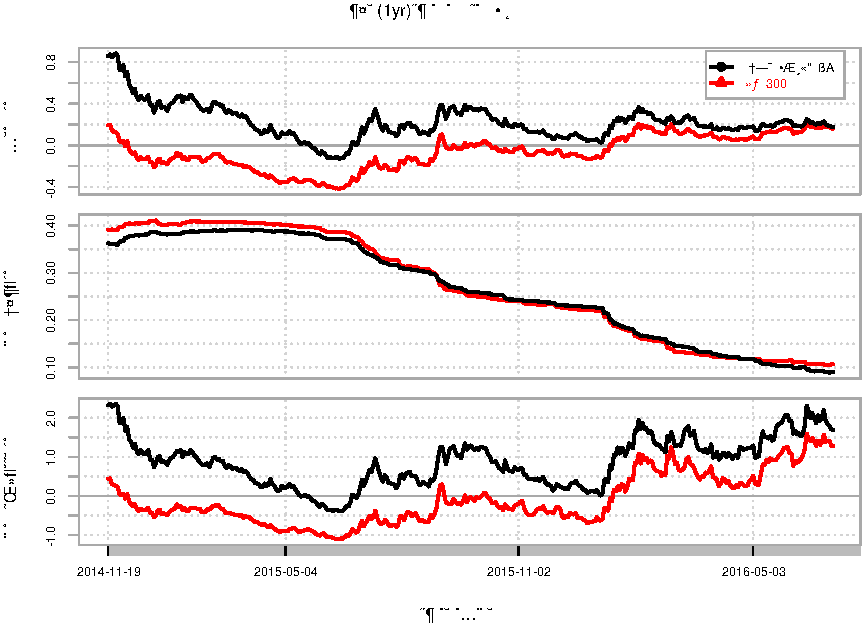
\includegraphics{hl-review_files/figure-latex/unnamed-chunk-3-1.pdf}
\caption{投资者收益风险比较}
\end{figure}

\section{简介}

上海财经大学金融学硕士,现任圆信永丰基金管理有限公司首席投资官。历任新疆金新信托证券管理总部信息研究部经理,德恒证券信息研究部副总经理,德恒证券经纪业务管理总部副总经理,兴业证券股份有限公司理财服务中心首席理财分析师,兴业证券股份有限公司上海资产管理分公司副总监。

\section{\texorpdfstring{风格与能力评价\footnote{运气能够带来超常表现,持续的好运则可以归结为能力!}}{风格与能力评价}}

作为首席投资官,洪流与他旗下基金经理们一起管理了多种不同类型的基金产品,在此过程中体现了洪流具备的如下风格与能力:

\begin{itemize}
\tightlist
\item
  尽管洪流自身是长线价值投资者,但是他驾驭不同投资风格的能力;
\item
  创新的产品设计与策略设计能力;
\item
  深度行业分析能力带来了行业配置收益;
\item
  熟练、细致的企业分析带来较强的股票选择能力。
\end{itemize}

\section{投资方法体系}

\subsection{股市中的绝对收益}

利用动态投资策略,在股市中获取绝对收益:

\begin{itemize}
\item
  用1-3个月的时间,低于20\%的股票仓位,利用无风险收益和股票市场中确定性比较的机会累计初始安全垫
\item
  当净值\(\geq 1.05\),增加仓位,同时提高安全垫的标准(即提高止损的标准,如净值1.03)
\end{itemize}

如此,实现了累计收益阶梯式的增长并有效的控制回撤,虽然不见得获得了最大的投资收益,但是收益风险比一定是靓丽的。

\subsection{投资研究方法}

\begin{itemize}

\item 战略判断(实际是中观分析),包括:
\begin{enumerate}
\item 行业周期:判断行业是否景气
\item 企业家精神:判断核心管理者的素质和团队战略管理方面的质量
\item 当前赛道的判断:长期的毛利水平,是否适应新的发展等
\end{enumerate}
\item 核心股票池跟踪(100个左右),要求
\begin{enumerate}
\item 持续的可预见的盈利增长
\item 拥有完整的数据链以支持研究判断
\item 月报、季报细致比较,动态跟踪风险收益比。
\end{enumerate}
\end{itemize}

\section{评价}

洪流是资深的投资人。他具备数学本科的背景,工作经历上提供了完整的管理能力、资产配置能力与资管能力的训练,同时形成了一个强大的朋友圈,这些都成为他投资上不可或缺的资源。我们基于公开信息,进行深度的科学分析,结合与其面对面的交流,做出如下评判:

\begin{enumerate}
\def\labelenumi{\arabic{enumi}.}
\tightlist
\item
  洪流有偏好长期价值,但是同时能够驾驭多种不同风格的基金管理者;
\item
  洪流有着成熟的行业分析方法和经验,能够从行业轮动中获取配置的机会,因而具备较好的行业配置的能力;
\item
  洪流具备了足够的经历去理解分析企业管理层,从而能够结合行业分析选取出好的投资标的,因此具备较强的择股能力;
\item
  当前的工作需要并没有挑战他的大类资产配置能力,我们只能说,洪流没有展示出大类资产配置的能力。
\end{enumerate}

因此,洪流是有着丰富的经历和阅历,具备深度行业分析与配置能力,较强的择股能力的基金管理者;同时他也具备强大的气质和管理经验,是一位成熟的基金经理的经理。

\begin{acknowledgement}

在我们的分析中,使用了公开数据与部分非公开数据,在此基础上采用基于净值的风格分析,基于持仓的收益归因对基金管理人的业绩表现进行了科学的分析。我们历尽所能的使用了最为完整与详实的数据、最为科学的方法,以最为严谨的态度做出尽量客观的评价。同时我们也实地进行调研与基金经理人进行了多次的交流。在此,对于向我们提供数据与交流机会的相关人员致谢。需要根伟详细的技术分析报告,请与本文作者联系。

\end{acknowledgement}
\end{document}
